\section{Support Vector Clustering}
\subsection{How it works in kernel space?}
\begin{frame}{How it works}
\begin{block}{In a mysterious space...}
Data points can be structured into a hypersphere where low density points are fading away.
\end{block}
\vskip20pt
\begin{figure}
\centering
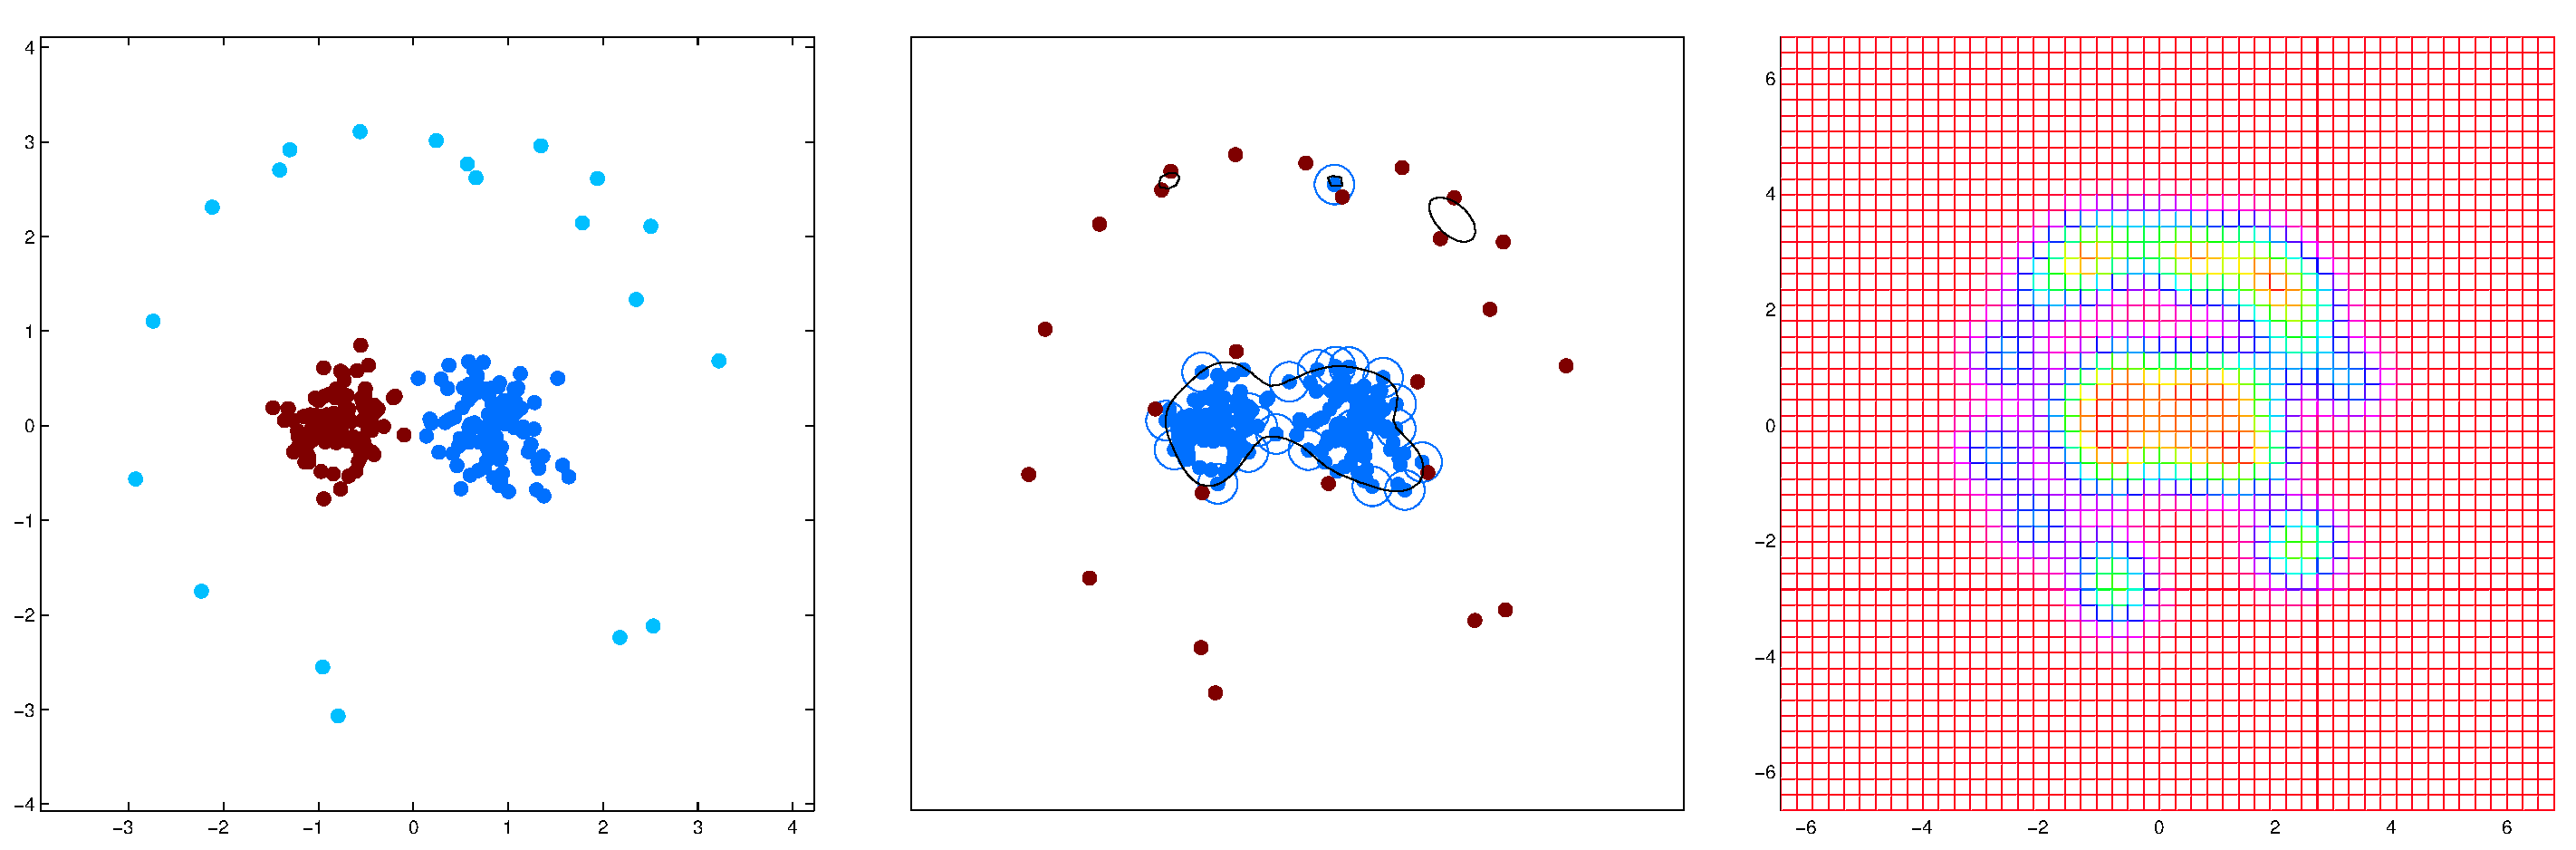
\includegraphics[scale=0.22]{imgs/svn_sample}
\caption{Support vector clustering example}
\end{figure}
\end{frame}

\begin{frame}{Cutting the low density area}
\begin{columns}
\begin{column}{.5\textwidth}
Support Vector Machine
\begin{figure}
\hskip-30pt
\includegraphics[scale=0.35]{imgs/svm_sample.pdf}
\end{figure}
\color{blue}Maximize the margin!
\end{column}
\begin{column}{.5\textwidth}
Support Vector Clustering
\begin{figure}
\hskip-30pt
\includegraphics[scale=0.2]{imgs/svc1.pdf}\\ \hskip-30pt
\includegraphics[scale=0.2]{imgs/svc1st.pdf}
\end{figure}
\color{blue}Minimize the hypersphere
\end{column}
\end{columns}
\end{frame}

\subsection{SVC Theory}
\begin{frame}{Optimization problem}
Looking for a smallest sphere $\left\langle R, g\right\rangle$ enclosing all data points:
\begin{align}
\label{eq:svc1}
&\min \left(R^2 + C\sum \xi_i\right)	\nonumber \\
\text{subject to}\quad &  \| \Phi(x_j) - g\|^2 \leq R^2 + \xi_j,\; \forall j \nonumber \\
& \xi_j \geq 0 \nonumber
\end{align} 
\begin{description}
\item[$R$]: the radius of the hypersphere
\item[$g$]: the center of the hypersphere
\item[$\| \Phi(x_j) - g\|^2$]: the distance of point $x_j$ to center $g$
\item[$\xi_i$]: slackness variables
\item[$C$]: punishments on slackness
\end{description}
\pause
\vskip20pt
\color{red} Minimizing the ball allowing part of points fade way (slackness).
\end{frame}

\begin{frame}{Properties}
\begin{columns}
\begin{column}{0.65\textwidth}
\begin{itemize}
\item The minimal ball with $R$ is cutting the data points from low density area.
\item Normal data points are inside the ball.
\item Support vectors $X_{SVs}$ are directly on the sphere.
\item Outliers with $\xi_i > 0$ is outside the ball.
\item The clustering bound is a natural threshold finding out the outliers. 
\item No need to define the $m$ (\#clusters)
\end{itemize}
\end{column}
\begin{column}{.35\textwidth}
\begin{figure}
\hskip-20pt
\includegraphics[scale=0.3]{imgs/svc3.pdf}
\end{figure}
\end{column}
\end{columns}
\end{frame}


\subsection{Connection to KDE}
\begin{frame}{From the cluster bound to centers}
\begin{figure}
\centering
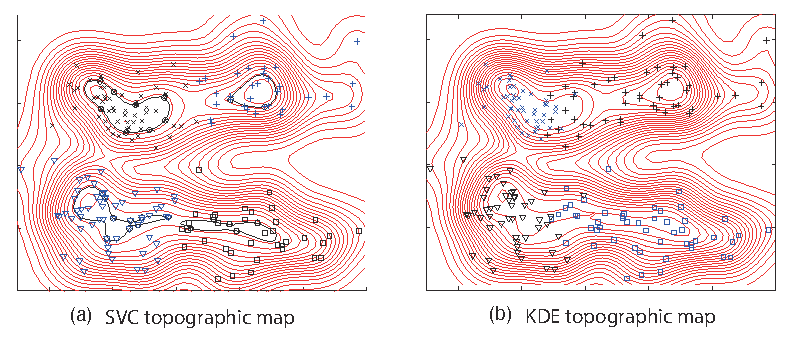
\includegraphics[scale=0.7]{imgs/svc_kde.pdf}
\end{figure}
\begin{itemize}
\item Shrink the cluster bounds to centers.
\item Allow all the points to be repelled outside the ball.
\end{itemize}
\end{frame}
\begin{frame}{Advantages over KDE}
\begin{itemize}
\item Computational easier
\item Define a core region rather than a peak
\item Topographically more reliable
\item Global optimal solution rather than many local maxima  
\end{itemize}
\end{frame}

\subsection{Open problems}
\begin{frame}{Optimization results}
Finally we got...
\vskip10pt
\[
g=\sum\beta_{\mathrm{sv}}\Phi(x_{\mathrm{sv}}) + \sum\beta_{\mathrm{bsv}}\Phi(x_{\mathrm{bsv}}) + \sum\beta_{\mathrm{in}}\Phi(x_{\mathrm{in}}),
\]
\begin{center}
$0 < \beta_{\mathrm{sv}} < C$, $\beta_{\mathrm{bsv}}=C$, $\beta_{\mathrm{in}}=0$
\end{center}
\pause
\vskip40pt
\color{red} Note: the ball center $g$ is still heavily biased by outliers ($\beta_{\mathrm{bsv}}$)
\end{frame}
\begin{frame}{Problems}
\begin{itemize}
\item Only deal with low density outliers
\item Learning is not robust ($g$ is biased)
\item We need to integrate user feedbacks
\end{itemize}
\end{frame}
%\begin{frame}{Statistical Implication}
%\begin{block}{Reichenbach's \textit{Common Cause Principle}}
%If $X$ and $Y$ are correlated, then either $X$ causes $Y$ or $Y$ causes $X$ or they share a latent common cause $Z$.
%\end{block}
%\begin{figure}
%\setcounter{subfigure}{0}
%	\centering
%	\begin{subfigure}[H]{0.3\textwidth}
%		\centering
%		\includegraphics[scale=0.3]{imgs/x2y}
%		\caption{$X$ causes $Y$}
%		%\label{}	
%	\end{subfigure}
%	\begin{subfigure}[H]{0.3\textwidth}
%		\centering
%		\includegraphics[scale=0.3]{imgs/y2x}
%		\caption{$Y$ causes $X$}
%		%\label{}	
%	\end{subfigure}
%	\begin{subfigure}[H]{0.3\textwidth}
%		\centering
%		\includegraphics[scale=0.3]{imgs/z2xy}
%		\caption{A common latent cause $Z$}
%		%\label{}	
%	\end{subfigure}
%\end{figure}\pause
%\begin{itemize}
%\item<+-|alert@+> It links causality with probability
%\end{itemize}
%\end{frame}
%\begin{frame}{Functional Causal Model (pearl et al.)} 
%\begin{itemize}[<+->]
%\item A set of variables (factors) $\left\lbrace X_1,\ldots,X_n \right\rbrace$
%\item Directed acyclic graph $\mathcal{G}$ with vertices $\left\lbrace X_1,\ldots,X_n \right\rbrace$
%\item Parents of node $X_i$ in $\mathcal{G}$ are its direct causes
%\item $X_i=f_i(Parents(X_i),\epsilon_i)$, where $\left\lbrace\epsilon_1,\ldots,\epsilon_n\right\rbrace$ are jointly independent noises
%\item The above entails a joint probability distribution $P(X_1,\ldots,X_n)$
%\item Problems are twofold:
%      \begin{enumerate}
%		\item How is the $P$ like?
%		\item Can we recover $\mathcal{G} from P$? 
%	\end{enumerate}
%\item[] \begin{textblock*}{200mm}(0.6\textwidth,-2cm)
%		\includegraphics[scale=0.25]{imgs/causalgm}
%	\end{textblock*}
%\end{itemize}
%\end{frame}
%\begin{frame}{Functional Causal Model, ctd.}
%The following are equivalent:
%\begin{itemize}
%\item A functional causal model exists
%\item Local causal Markov condition: $X_i$ is statistically independent of its non-descendants given $X_i$'s parents
%\item Global Causal Markov condition: \textbf{d-separation} characterize the set of independences over all the observables
%\item Factorization: $P(X_1,\ldots,X_n)=\prod_iP(X_i\,|\,Parents(X_i))$
%\end{itemize}
%\end{frame}
%\begin{frame}{Learning causation from Data?}
%\begin{block}{Question}
%Given observational data, can we infer $\mathcal{G}$?
%\end{block}
%\begin{itemize}
%\item \textbf{Simple answer:} impossible without additional information
%\item Possible with interventions (outside force, empirical treatment, etc.)
%\item By conditional independence tests, \textit{Markov equivalence class} containing $\mathcal{G}$ can be learned. \alert{But}, it fails in simplest 2-nodes case.
%\item 2-nodes case can be tackled applying residual dependence test. (see Hoyer et al.)
%\end{itemize}
%\end{frame}
%\begin{frame}{Markov Equivalence Class}
%\textbf{Simplest case with three variables}
%\begin{itemize}
%\item[]<1-> \begin{figure}
%\setcounter{subfigure}{0}
%			\begin{subfigure}[H]{0.4\textwidth}
%			\includegraphics[scale=0.4]{imgs/eqv}
%			\caption{Equivalence}
%			\end{subfigure}\hfill
%			\begin{subfigure}[H]{0.3\textwidth}
%			\includegraphics[scale=0.4]{imgs/noneqv}
%			\caption{Non-equivalence}
%			\end{subfigure}
%		\end{figure}
%\item<2-> Samples can be explained by all graphs in equivalence class
%\item<3-> For example:
%\begin{table}
%\centering
%\begin{tabular}{|c|c|}
%\hline
%Equivalence class & Non-equivalence class \\\hline
%$Dep(X,Z\,|\,\emptyset)$ & $Dep(X,Z\,|\,\emptyset)$\\\hline
%$Dep(Y,Z\,|\,\emptyset)$ & $Dep(Y,Z\,|\,\emptyset)$\\\hline
%$Dep(X,Y\,|\,\emptyset)$ & \alert{$Ind(X,Y\,|\,\emptyset)$}\\\hline
%$Ind(X,Y\,|\,Z)$ & \alert{$Dep(X,Y\,|\,Z)$}\\\hline
%\end{tabular}
%\end{table}	
%\end{itemize}
%\end{frame}